\documentclass[a4paper, 12pt]{article}
\usepackage[a4paper,top=1.5cm, bottom=1.5cm, left=1cm, right=1cm]{geometry}
\usepackage{cmap}					
\usepackage{mathtext} 				
\usepackage[T2A]{fontenc}			
\usepackage[utf8]{inputenc}			
\usepackage[english,russian]{babel}
\usepackage{multirow}
\usepackage{graphicx}
\usepackage{wrapfig}
\usepackage{tabularx}
\usepackage{float}
\usepackage{longtable}
\usepackage{hyperref}
\hypersetup{colorlinks=true,urlcolor=blue}
\usepackage[rgb]{xcolor}
\usepackage{amsmath,amsfonts,amssymb,amsthm,mathtools} 
\usepackage{icomma} 
\usepackage{euscript}
\usepackage{mathrsfs}
\usepackage{enumerate}
\usepackage{caption}
\usepackage{enumerate}
\mathtoolsset{showonlyrefs=true}
\usepackage{graphicx}
\usepackage{caption}
\usepackage{subcaption}
\usepackage{amsthm}
\usepackage[europeanresistors, americaninductors]{circuitikz}
\DeclareMathOperator{\sgn}{\mathop{sgn}}
\newcommand*{\hm}[1]{#1\nobreak\discretionary{}
	{\hbox{$\mathsurround=0pt #1$}}{}}

\newcommand{\framedtext}[1]{%
\par%
\noindent\fbox{%
    \parbox{\dimexpr\linewidth-2\fboxsep-2\fboxrule}{#1}%
}%
}

\title{\textbf{Измерение коэффициента поверхностного натяжения жидкости (2.5.1)}}
\author{Манро Эйден}
\date{}

\begin{document}

\maketitle

\begin{center}
    \section*{Введение}
\end{center}

\noindent \textbf{Цель работы:} 1) измерение температурной зависимости  коэффициента поверхностного натяжения дистиллированной воды с использованием известного коэффициента поверхностного натяжения спирта; 2) определение полной поверхностной энергии  и теплоты, необходимой для изотермического образования единицы поверхности жидкости  при различной температуре.

\bigskip

\noindent \textbf{Оборудование:} прибор  Ребиндера  с термостатом и микроманометром; исследуемые жидкости; стаканы.

\bigskip

\begin{center}
    \subsection*{Теоретические сведения}
\end{center}

Наличие поверхностного слоя приводит к разнице давлений по разные стороны от искривленной границы раздела двух сред. 
Для сферического пузырька с воздухом внутри жидкости избыточное давление рассчитывается с использованием формулы Лапласа,

\begin{equation} \label{laplas}
    \Delta P = \frac{2\sigma}{r}
\end{equation}

где $\sigma$  – коэффициент поверхностного натяжения, $P_{\text{внутри}}$ и $P_{\text{снаружи}}$ – давление внутри пузырька и снаружи, $r$ – радиус кривизны поверхности раздела двух фаз. Эта формула является основой предложенного метода определения коэффициента поверхностного натяжения жидкости. Для этого измеряется давление $\varDelta P$, необходимое для выталкивания в жидкость пузырька воздуха.

\begin{center}
    \subsection*{Экспериментальная установка}
\end{center}

\begin{figure}[H] 
    \center{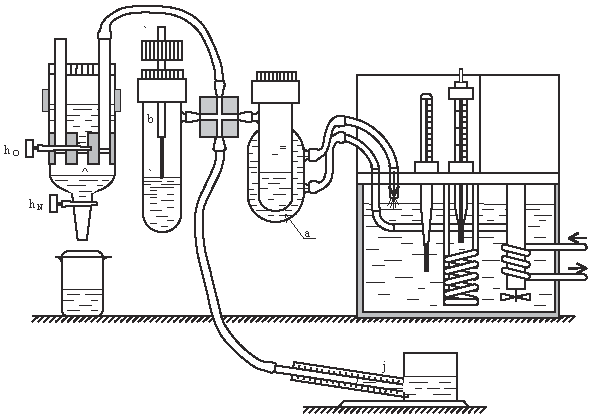
\includegraphics[scale=1]{img/ustanovka.pdf}}
    \caption{Схема установки для измерения температурной зависимости коэффициента поверхностного натяжения.}
    \label{ris:ustanovka}
\end{figure}

Исследуемая жидкость (дистиллированная вода) наливается в сосуд (колбу) \textbf{В} (рис. \ref{ris:ustanovka}). Тестовая жидкость  (этиловый спирт) наливается  в сосуд \textbf{E}. При измерениях  колбы герметично закрываются  пробками.   Через одну из двух пробок  проходит полая металлическая игла \textbf{C}. Этой пробкой закрывается сосуд, в котором  проводятся измерения. Верхний конец иглы открыт в атмосферу, а нижний погружен в жидкость. Другой сосуд герметично закрывается второй пробкой. При создании достаточного  разряжения воздуха в колбе с иглой пузырьки воздуха начинают пробулькивать через жидкость. Поверхностное натяжение можно определить по величине разряжения $\Delta P$ (\ref{laplas}), необходимого для прохождения пузырьков (при известном радиусе иглы).\\
Разряжение в системе создается с помощью аспиратора \textbf{A}. Кран \textbf{K2} разделяет две полости аспиратора. Верхняя полость при закрытом кране \textbf{K2}  заполняется водой. Затем кран \textbf{K2} открывают и заполняют водой  нижнюю полость  аспиратора.  Разряжение воздуха создается в нижней полости  при открывании крана \textbf{K1}, когда  вода вытекает из неё по каплям. В колбах \textbf{B} и \textbf{C}, соединённых трубками с нижней полостью аспиратора,  создается такое же пониженное давление. Разность давлений в полостях с разряженным воздухом и атмосферой измеряется спиртовым микроманометром.

\bigskip

\begin{center}
    \subsection*{Погрешности}
\end{center}

\begin{center}
    \item $\sigma_{\text{микроскоп}} = 0,05 \; \text{мм}$ \; $\sigma_{\text{линейка}} = 0,5 \; \text{мм}$ \; $\sigma_{\text{манометр}} = 0,1 \; \text{Па} $ 
\end{center}

    
\newpage


\begin{center}
    \section*{Ход работы}
\end{center}

\subparagraph{1.} Проверим герметичность установки. 

\subparagraph{2.} Откроем кран К1. Подберём частоту падения капель около одной капли в 5 секунд. 

\subparagraph{3.} Измерим максимальное давление $\Delta P_{\text{спирт}}$  при  пробулькивании пузырьков воздуха через спирт. Данные занесём в таблицу 1. По разбросу результатов оценим случайную погрешность измерения. 

\begin{table}[h!]
    \centering
    \begin{tabular}{|c|c|c|c|c|c|c|c|c|c|c|} \hline

        $N$             & 1  & 2  & 3  & 4  & 5  & 6  & 7  & 8  & 9  & 10  \\ \hline
        $h$, \text{дел} & 46 & 45 & 46 & 45 & 45 & 45 & 45 & 45 & 45 & 45  \\ \hline
        \multicolumn{11}{|l|}{$h_{\text{ср}} = 45,2$ \text{дел} \hspace{125} $\sigma_h = 0,3$ \text{дел}} \\ \hline
        
    \end{tabular}
    \caption{Измерения для спирта ($h_{\text{сп}}$)}
\end{table}

В таблице учтена только случайная погрешность величины $h$, которая составляет около $0,7 \; \%$  в то время как приборная погрешность составляет две цены деления (1 деление -- инструментальная погрешность и плюс ещё одно -- моя реакция и способность зафиксировать правильное деление), то есть её относительный вклад $\approx 2 / 46   \approx 4.3\%$.

По формуле $\Delta P_{\text{спирт}} = 0.2 \cdot 9.81 \cdot h$ вычислим $\Delta P_{\text{спирт}}$.

\bigskip

\begin{center}
    \underline{ $\Delta P_{\text{спирт}} = (88.7\pm 3.8) \; \text{Па}$}
\end{center}
    
    


\end{document}